\section{Three Learning Principles}
\noindent
{\color{LightRubineRed} \rule{\linewidth}{1mm} }
%%%%%%%%%%%%%%
\subsection{Occam's Razor} % (fold)
\label{sub:occam_s_razor}
\begin{myremark}{}
\Large{Simple is Better !!}
\end{myremark}
The simplest model that fits the data is also the most plausible. \par
% subsection occam_s_razor (end)

\subsection{Sampling Bias} % (fold)
\label{sub:sampling_bias}
\begin{myremark}{}
\Large{iid is importance !!}
\end{myremark}
If the data is sampled in biased way,learning will produce a similarly biased outcome. \par
\textcolor{mypink2}{\Large{Match test scenario(distribution)}} as much as possible.
% subsection sampling_bias (end)

\subsection{Data Snooping} % (fold)
\label{sub:data_snooping}
偷看数据很严重。 \par
\begin{center}
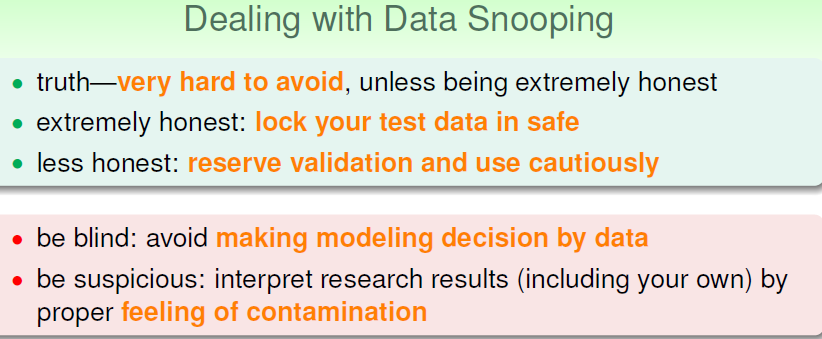
\includegraphics[width=10cm, height=4cm]{lecture16_1}
\end{center}
% subsection data_snooping (end)

\subsection{Three Related Fields} % (fold)
\label{sub:three_related_fields}
\begin{center}
\Large{Three Related Fields} \par
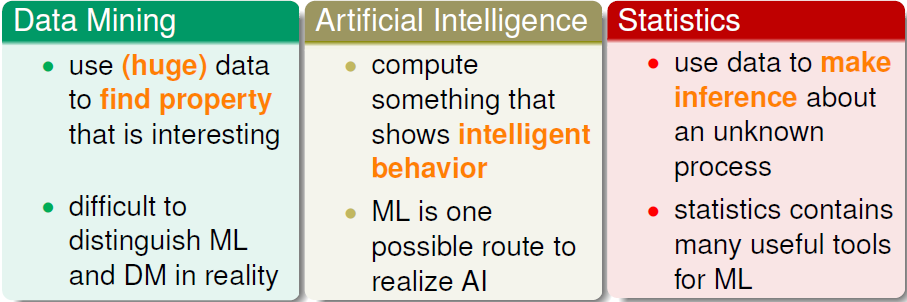
\includegraphics[width=14cm, height=5cm]{lecture16_2}
\end{center}

\begin{center}
\Large{Three Theoretical Bounds} \par
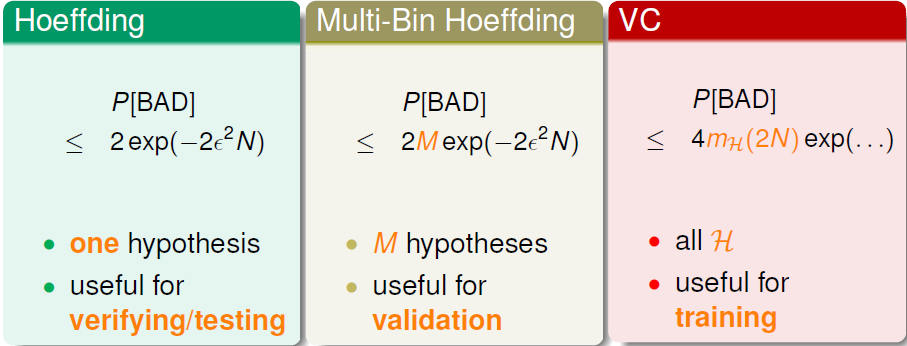
\includegraphics[width=14cm, height=5cm]{lecture16_3}
\end{center}

\begin{center}
\Large{Three Linear Models} \par
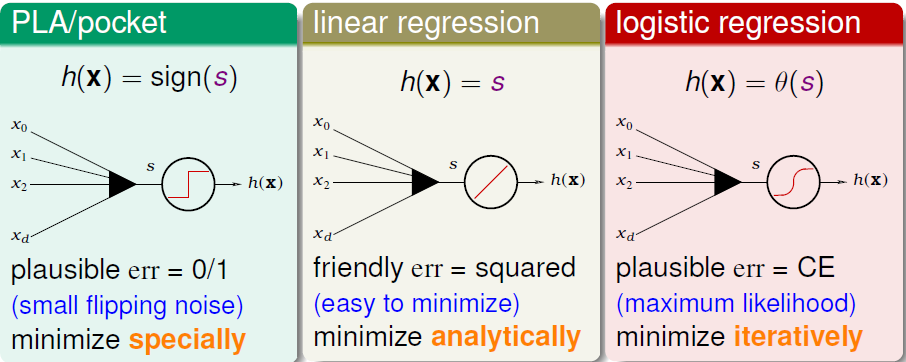
\includegraphics[width=14cm, height=5cm]{lecture16_4}
\end{center}

\begin{center}
\Large{Three Key Tools} \par
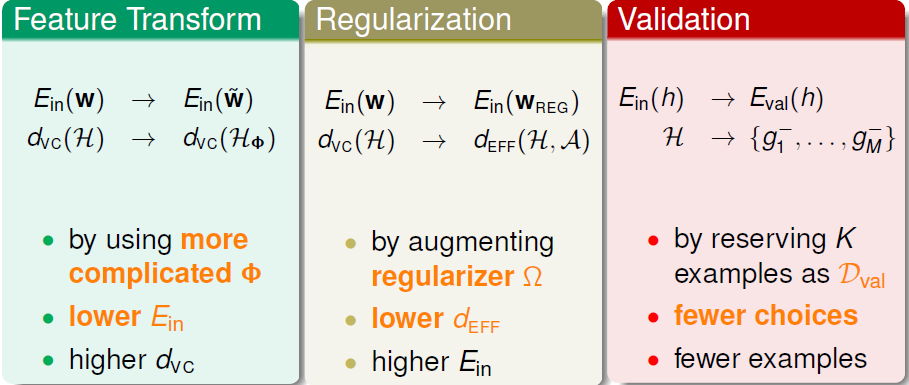
\includegraphics[width=14cm, height=5cm]{lecture16_5}
\end{center}

\begin{center}
\Large{Three Learning Principles} \par
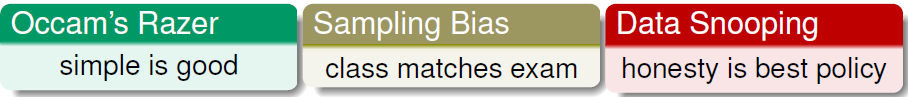
\includegraphics[width=14cm, height=2cm]{lecture16_6}
\end{center}
% subsection three_related_fields (end)
%%%%%%%%%%%%%%
\begin{center}
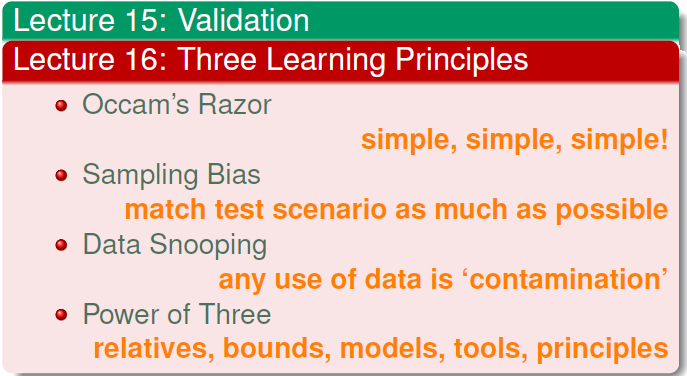
\includegraphics[width=14cm, height=5cm]{lecture16_sum}
\end{center}
\noindent
{\color{RubineRed} \rule{\linewidth}{1mm} }